\documentclass[12pt,a4paper]{article}
\usepackage[utf8]{inputenc}
\usepackage[provide=*]{babel}
\babelprovide[import=de, main]{de}
\usepackage[T1]{fontenc}
\usepackage{geometry}
\geometry{a4paper, left=2.5cm, right=2.5cm, top=3cm, bottom=3cm}
\usepackage{graphicx}
\usepackage{hyperref}
\usepackage{tikz}
\usetikzlibrary{shapes.geometric, arrows.meta, positioning, fit, backgrounds}
\usepackage{enumitem}
\usepackage{tabularx}
\usepackage{xcolor}
\usepackage{amsmath}
\usepackage{float}


\title{\textbf{Arbeitsexposé}\\KI-gestützte 3D-Rekonstruktion linearer Infrastruktur: Evaluierung einer Docker-basierten Scan-to-BIM Pipeline mittels SAM 3 und Gaussian Splatting}
\author{Bachelor- und Projektarbeit}
\date{\today}

\begin{document}

\maketitle

\section{Einleitung und Forschungsfrage}
Die präzise Erfassung schwer zu modellierender, extrem dünner Objekte (wie Stromerdkabel in Baugräben) stellt für klassische photogrammetrische Verfahren (SfM) eine große Herausforderung dar. Ziel dieser Arbeit ist die Entwicklung und Evaluierung eines "Scan-to-BIM"-Workflows, der die Vorzüge der 2D-KI-Segmentierung (Segment Anything Model 3) mit modernsten 3D-Rekonstruktionsmethoden (3D Gaussian Splatting via SuGaR) verbindet.

Wie aktuelle Forschungen belegen, erzeugen 3D Gaussian Splatting Algorithmen durch mathematische Wahrscheinlichkeitsfunktionen hochgradig detailreiche, fotorealistische Visualisierungen bei geringer Rechenlast. Sie werden zunehmend im Ingenieurwesen und zur Generierung von Orthofotos (z.B. Integration in ArcGIS Pro) eingesetzt. Jedoch fehlt 3DGS-Modellen die inhärente Georeferenzierung.
Die zentrale Forschungsfrage lautet daher: \textit{Lässt sich die 3D-Rekonstruktion linearer Infrastruktur durch eine vorgelagerte 2D-Segmentierung und ein objektspezifisches 3DGS-Training (Segment-then-Splat) so optimieren und georeferenzieren, dass strenge ingenieurstechnische Toleranzen eingehalten werden?}

\section{Praxisbezug und Erfolgskriterien}
Die Pipeline wird direkt für den Anwendungsfall der TenneT (Übertragungsnetzbetreiber) konzipiert.
\begin{itemize}
    \item \textbf{Geometrische Toleranz:} Eine Abweichung von maximal $\pm$ 10\,cm in Lage und Höhe gegenüber der realen Kabeltrasse.
    \item \textbf{Georeferenzierung \& GIS-Integration:} Das finale 3D-Modell muss präzise in einem UTM-Koordinatensystem vorliegen, um den direkten Import in Geoinformationssysteme (z.B. ArcGIS Pro) zu gewährleisten.
    \item \textbf{Wirtschaftliche Evaluierung:} Eine Kostengegenüberstellung des Drohnen- und Serverrechenaufwands im Vergleich zur klassischen, terrestrischen Vermessung.
\end{itemize}

\section{Methodik und Architektur (Workflow v3)}
Der Ansatz basiert auf einer klaren Trennung von 2D-Bildverarbeitung und 3D-Meshing.

\subsection{Software-Repositories}
\begin{itemize}
    \item \textbf{SAM 3 (Meta):} Zuständig für Concept-Prompting und Video-Tracking.
    \item \textbf{COLMAP:} Generierung der Kameraposen auf Basis der \textit{unmaskierten} Originalbilder. Die Pipeline nutzt ausschließlich das schnelle \textit{Structure from Motion} (SfM) von COLMAP. Die rechenintensive dichte Rekonstruktion (MVS) wird vollständig übersprungen.
    \item \textbf{Segment-then-Splat (STS):} Übernimmt das objektspezifische 3DGS-Training (Lu et al., NeurIPS 2025). STS teilt die initialen COLMAP-Gaussians anhand der SAM 3 Masken in objektspezifische Sets auf und trainiert diese mit einem dedizierten Object-specific Loss ($\mathcal{L}_{obj}$), ohne die Ground-Truth-Bilder zu manipulieren. Das Ergebnis ist ein vollständiges 3DGS-Modell, in dem jeder Gaussian eine Object-ID trägt. SAM 3 ersetzt hierbei das intern vorgesehene AutoSeg-SAM2.
    \item \textbf{SuGaR:} Surface extraction with Gaussian Splatting. Übernimmt den vortrainierten STS-Checkpoint und wendet geometrische Regularisierung (DN-Consistency, Normal Alignment) sowie Poisson Surface Reconstruction an. SuGaR zwingt die von STS bereits sauber zugewiesenen Gaussians dazu, sich flach an die reale 3D-Oberfläche anzuschmiegen, und extrahiert daraus ein hochqualitatives Mesh.
    \item \textbf{DGtal:} Open-Source Geometrie-Bibliothek zur finalen Centerline-Extraktion. Sie wandelt die Oberfläche des Kabel-Sub-Meshes in eine räumliche 1D-Kurve (Centerline bzw. Scheitelachse mit lokalen Koordinaten) um.
\end{itemize}

\subsection{Pipeline-Struktur: Temporale Konsistenz vs. SAHI}
Für die Erkennung extrem dünner Kabel in hochauflösenden 4K-Bildern bietet sich theoretisch \textit{Slicing Aided Hyper Inference} (SAHI) an. SAHI zerschneidet das Bild in kleinere Teilbereiche (Patches), wodurch verhindert wird, dass dünne Kabel beim Downscaling auf die native Modellauflösung von SAM 3 "verschluckt" werden.

Dennoch wurde der primäre Fokus für diese Pipeline bewusst auf den \textbf{SAM 3 Video Predictor} gelegt. Der methodische Nachteil von SAHI ist die fehlende temporale Konsistenz: Da SAHI jedes Einzelbild isoliert betrachtet, "flackern" die erzeugten Masken von Frame zu Frame, wenn sich Lichteinfall oder Blickwinkel leicht ändern. 3D Gaussian Splatting erfordert jedoch zwingend formstabile, konsistente Masken über alle Kameraperspektiven hinweg, da sonst fehlerhafte Artefakte in den 3D-Raum projiziert werden. Der SAM 3 Video Predictor löst dieses Problem durch ein Memory-Modul, welches die Kabel-Pixel über die Zeit hinweg verfolgt und dadurch flackerfreie, temporär konsistente Masken liefert. SAHI dient in dieser Pipeline lediglich als Fallback-Route für spezifische Bildausschnitte, in denen das temporale Tracking abreißen sollte.


\section{Docker-Infrastruktur und Orchestrierung}
Ein Kernproblem moderner KI-Pipelines sind tiefgreifende Versionskonflikte zwischen den benötigten Nvidia-Grafikkartentreibern (CUDA). Dieses Problem wird durch eine \texttt{docker-compose} Architektur vollständig gelöst. Die Pipeline isoliert die Anwendungen in voneinander getrennte Container, während alle erzeugten Daten über \textbf{Docker Bind Mounts (Volumes)} zentral und persistent auf dem Host-System (Windows/Linux) gespeichert werden.

Um die Automatisierung zu maximieren, wird die Pipeline über ein zentrales Master-Skript (\textit{One-Click-Orchestration}) gesteuert. Dieses Skript stößt die Container sequenziell an, muss jedoch für manuelle Arbeitsschritte pausieren. Es kommen fünf dedizierte Container zum Einsatz:
\begin{itemize}
    \item \textbf{Container A (Vorverarbeitung):} Beinhaltet PyTorch 2.x und SAM 3. Benötigt das Nvidia Container Toolkit (CUDA >= 12.6).
    \item \textbf{Container B (SfM):} Ein offizielles NVIDIA-Image für COLMAP (CUDA 11.8 oder 12.1). \textit{Nach Ausführung dieses Containers pausiert das Master-Skript automatisch (Breakpoint). Der Nutzer öffnet CloudCompare auf dem Host-System, pickt die GCPs und speichert die Transformationsmatrix. Anschließend wird das Skript mit ``Enter'' fortgesetzt.}
    \item \textbf{Container C (Object-specific 3DGS):} Beinhaltet Segment-then-Splat (STS). Empfängt die SAM 3 Masken und die COLMAP-Kameraposen und führt das objektspezifische 3DGS-Training mit dem nativen Object-specific Loss ($\mathcal{L}_{obj}$) durch. Benötigt CUDA 12.1 (PyTorch 2.3.1). SAM 3 ersetzt hierbei das intern vorgesehene AutoSeg-SAM2 als Masken-Frontend.
    \item \textbf{Zwischenschritt 3.5 (Kabel-Isolierung):} Ein dediziertes Python-Skript \texttt{filter\_cable\_pc.py} filtert die dichte STS 3D-Punktwolke direkt vor der Übergabe an das Meshing-Tool. Es extrahiert gezielt die Kabel-Vordergrund-Splats (Standardwert auf mittlerer Ebene \texttt{obj\_id\_m == 1}) und verwirft alle Hintergrundpunkte, um SuGaR-Artefakte (schwarze Floating-Wolken) drastisch zu reduzieren.
    \item \textbf{Container D (Meshing):} Beinhaltet SuGaR. Lädt den gefilterten, isolierten Kabel-Checkpoint und wendet die geometrische Regularisierung (DN-Consistency) sowie Poisson Surface Reconstruction an. Wegen tiefer Abhängigkeiten zum \texttt{diff-gaussian-rasterization} Modul wird hier strikt CUDA 11.8 erzwungen. Das intern geforderte Conda-Environment wird systemweit über eine Anpassung der \texttt{ENV PATH} Variable im Dockerfile nativ zugänglich gemacht.
    \item \textbf{Container E (Post-Processing):} Ein reiner \textbf{CPU-Container} (ohne GPU/CUDA-Abhängigkeit). Beinhaltet die C++ Bibliothek DGtal sowie die GDAL-Tools (\texttt{ogr2ogr}). Durch die Auslagerung dieser CPU-basierten Nachbearbeitung in einen eigenen Microservice bleibt die Architektur extrem leichtgewichtig, da keine massiven Nvidia-Images geladen werden müssen.
\end{itemize}

\section{Risikomanagement und Datenhandling}
Vier kritische Punkte erfordern besondere Aufmerksamkeit:
\begin{enumerate}
    \item \textbf{Speichermanagement:} Drohnenvideos in 4K bei 60 FPS erzeugen massive Datenmengen. Das Konzept sieht vor, dass diese temporär im nativen Linux-Dateisystem liegen und nach der 6 FPS Extraktion gelöscht werden, um I/O-Engpässe unter WSL2 zu vermeiden.
    \item \textbf{SAM 3 Tracking-Stabilität (VRAM) und Modellkonsistenz:} \\
          In der praktischen Ausführung zeigte sich ein nichtlinear wachsender VRAM-Bedarf im \texttt{propagate\_in\_video}-Pfad (insb. während \texttt{F.interpolate} in der Output-Erzeugung). Dadurch trat ein \texttt{CUDA out of memory} nicht deterministisch auf (z. B. um Frame 45, bei anderen Läufen früher oder später), obwohl dieselbe Eingabe verwendet wurde. Ursache ist die Kombination aus langem Sequenzgedächtnis (Memory-Modul), fragmentiertem Allocator-Zustand und voller HD-Auflösung über viele Frames. \\
          Als technische Gegenmaßnahme wurde die Propagation auf feste Zeitfenster (Chunking) umgestellt: Jeder Lauf verarbeitet nur ein Segment mit \texttt{start\_frame\_index} und \texttt{max\_frame\_num\_to\_track}; die Masken werden unmittelbar pro Frame persistiert, statt alle Outputs bis zum Ende im RAM/VRAM vorzuhalten. Zusammen mit Offloading-Flags (Video/State auf CPU) stabilisiert dies die Pipeline auf 16-GB-Karten. \\
          Ein zweiter, davon getrennter Befund ist die \textbf{Gewichts-/Architektur-Konsistenz}: Trotz stabilem Lauf können aufgrund von \texttt{Missing keys}/\texttt{Unexpected keys} beim Laden des SAM-Checkpoints formal gültige, aber inhaltlich leere Masken entstehen. Daher wird als Quality-Gate vor Übergabe an STS verbindlich geprüft: (i) Anteil nichtleerer Masken, (ii) temporale Kontinuität über benachbarte Frames, (iii) Sichtprüfung an Stichproben. Nur bei erfüllten Kriterien werden Masken in Container C übernommen.
        \item \textcolor{blue}{\textbf{[GELÖST: SAM 3.1 Video-Tracking stabilisiert, Stand 06/2026]}} \\
            Die anfängliche Instabilität des SAM 3.1 Video-Pfades konnte durch drei gezielte Maßnahmen gelöst werden, was eine unterbrechungsfreie Voll-Propagation über alle 100 Frames auf einer 16-GB-GPU ermöglichte:
            (i) \textbf{VRAM-Limitierung durch sequenzielles Vision-Language-Matching}: Die Aktivierung von \texttt{batched\_grounding\_batch\_size = 1} (anstelle von standardmäßigem Batching nach Text-Prompts) reduzierte den VRAM-Verbrauch von über 12\,GB auf unter 5\,GB, wodurch jegliche \texttt{CUDA out of memory}-Fehler verhindert wurden. Zusätzlich wurde die PyTorch-Compilation via \texttt{TORCH\_COMPILE\_DISABLE=1} deaktiviert, um massive RAM/VRAM-Spitzen vorzubeugen.
            (ii) \textbf{Behebung des Shape-Assertions-Fehlers}: Der zuvor auftretende Fehler \texttt{AssertionError: pos\_pred\_mask.shape[0] == 1} bei der Chunk-Verarbeitung wurde durch Rückkehr zum globalen Video-Inferenz-Modus unter Verwendung der Standard-Konditionierungsparameter (\texttt{max\_cond\_frames\_in\_attn} unlimitiert) gelöst.
            (iii) \textbf{Datensatz-Kompatibilität bei der Masken-Persistierung}: SAM 3.1 Multiplex liefert den Vorhersage-Stream nicht in Form geschachtelter Dictionaries wie reguläre SAM-Modelle, sondern im Multiplex-spezifischen Format, d.\,h. als Dictionary mit den Hauptschlüsseln \texttt{out\_obj\_ids} und \texttt{out\_binary\_masks}. Ein angepasster Masken-Parser extrahiert nun die Binärmasken direkt über \texttt{out\_binary\_masks[idx]}.
            Durch diese Korrekturen konnte die Inferenz bei ca. 3,1\,it/s vollständig stabilisiert werden und liefert mit dem Text-Prompt \texttt{"cable"} reproduzierbar \textbf{33 nicht-leere Masken} über den 100 Frames großen Testdatensatz hinweg. \\
            \textbf{Einfache Erklärung (für Laien/Nicht-Techniker verständlich):} \\
            Zuvor brach das System beim Versuch, das Kabel im Video automatisch zu verfolgen, ständig ab oder fand schlichtweg gar nichts. Das lag an drei anschaulichen Problemen:
            \begin{itemize}
                \item \textit{Die Speicher-Überlastung (VRAM-Absturz):} Das Programm wollte alle KI-Bildanalysen für die Text-Prompts gleichzeitig im Grafikspeicher lösen. Das ist so, als ob man versucht, 10 dicke Bücher gleichzeitig auf einmal aufzuschlagen und querzulesen -- das Gehirn (die GPU) ist überfordert. Indem wir dem System befehlen, die Sätze brav nacheinander zu verarbeiten (\texttt{Batch-Größe = 1}) und das zeitaufwendige „Vorab-Auswendiglernen“ ausschalten (\texttt{Kompilierung aus}), liest die GPU das Video nun stressfrei Bild für Bild. Der Speicherbedarf sank von über 12\,GB auf gemütliche 4,5\,GB.
                \item \textit{Die Denkblockade (Der AssertionError):} Um Speicher zu sparen, hatten wir das Video anfangs in kurze 8-Bild-Häppchen zerlegt. Die KI kam bei der Übergabe der Häppchen jedoch völlig durcheinander, verlor den Faden und behauptete stur, die Teile würden logisch nicht mehr zusammenpassen. Wir lassen das Video nun einfach elegant am Stück durchlaufen und überlassen der KI die vollautomatische Verwaltung ihres Langzeitgedächtnisses.
                \item \textit{Das Übersetzungs-Missverständnis (Leere Maskenergebnisse):} Die KI hat das Kabel im Video zwar erfolgreich gefunden und markiert, dies aber in einer neuen „fremden Sprache“ (einem veränderten Ausgabeformat) dokumentiert. Unser Empfänger-Skript suchte die Ergebnisse beharrlich am alten Ablageort und meldete fälschlicherweise „nichts gefunden“. Der neu geschriebene Parser übersetzt diese neue Struktur nun fehlerfrei, wodurch die erzeugten Kabelmasken exakt erfassungskonform abgespeichert werden können.
            \end{itemize}
        \item \textcolor{blue}{\textbf{[GELÖST: SAM 3.1 lauffähig nach Laufzeit-Modernisierung, Stand 06/2026]}} \\
            Die zuvor beschriebenen Lade- und Stabilitätsprobleme ließen sich auf eine \textbf{nicht explizit fixierte, zu niedrige Python-Laufzeit} (vormals Python 3.10) zurückführen. Da SAM 3.1 moderne Laufzeitkomponenten voraussetzt, kam es ohne explizite Versionsfestlegung wiederholt zu Import- und Kompatibilitätsfehlern, sodass die Umgebung erst nach mehreren Korrekturen wieder vollständig lief. Die Lösung war eine konsequente \textbf{Pinnung der gesamten Laufzeit} in Container A: \texttt{nvidia/cuda:12.6.3-cudnn-devel-ubuntu24.04} mit \textbf{Python 3.12}, \textbf{PyTorch 2.7.0+cu126} und \textbf{torchvision 0.22.0}. \\
            Drei konkrete Stolpersteine wurden dabei behoben: (i) Unter Ubuntu 24.04 verhindert die \textit{externally-managed-environment}-Richtlinie (PEP 668) eine direkte \texttt{pip}-Installation; dies erfordert das Flag \texttt{-{}-break-system-packages}. (ii) Beim Import des SAM-3.1-Pakets fehlten Laufzeitabhängigkeiten (\texttt{psutil}, \texttt{timm}), die explizit nachinstalliert werden mussten. (iii) Der Image-Pfad lädt standardmäßig das SAM-3-Gewicht; für SAM 3.1 muss der Checkpoint über \texttt{download\_ckpt\_from\_hf(version="sam3.1")} ausdrücklich angefordert werden. \\
            Ergänzend wurde ein \textbf{Einzelbild-Pfad} implementiert: Das Vorverarbeitungsskript erkennt nun automatisch, ob in \texttt{01\_raw} ein Standbild (\texttt{.jpg}/\texttt{.jpeg}/\texttt{.png}) oder ein Video (\texttt{.mp4}/\texttt{.mov}) vorliegt, und nutzt für Bilder den text-geprompteten \texttt{build\_sam3\_image\_model} mit \texttt{Sam3Processor}. Dieser Pfad konnte auf einer statischen Testaufnahme mit dem Prompt ``cable'' reproduzierbar eine nichtleere Maske erzeugen. Der beim Laden weiterhin protokollierte \texttt{missing\_keys}-Hinweis (vier \texttt{convs.3}-Einträge des Vision-Backbones) blieb dabei folgenlos und steht der Maskengenerierung nicht entgegen.
    \item \textbf{Das Georeferenzierungs-Paradoxon:} Da die objektspezifische Selektion (STS) nur das Kabel-Mesh isoliert, verschwinden im finalen 3D-Modell auch die am Boden ausgelegten Passpunkte (GCPs). Eine Post-Training Transformation des Modells durch manuelles Anklicken ist somit nicht anwendbar. Die Lösung ist eine \textit{Pre-Training Georeferenzierung}: Die Open-Source-Software \textbf{CloudCompare} bietet hierfür ein ideales GUI. Da CloudCompare intern mit 32-Bit Single-Precision-Gleitkommazahlen arbeitet, führt eine direkte Eingabe von großen globalen UTM-Koordinaten ($> 10^5$) zu dramatischem Präzisionsverlust ($1$--$10$\,cm). Daher wird eine \textit{relative Georeferenzierung} durchgeführt: Ein ausgewählter GCP dient als lokaler Ursprung (Ankerpunkt) mit den Koordinaten $(0,0,0)$, und alle anderen GCPs werden relativ zu diesem berechnet ($GCP_{\text{relativ}} = GCP_{\text{UTM}} - GCP_{\text{Anker}}$). Man lädt die unmaskierte, spärliche SfM-Punktwolke aus COLMAP in CloudCompare, ordnet die Passpunkte den relativen GCP-Koordinaten manuell zu (\textit{Point Picking}) und berechnet eine 4x4-Transformationsmatrix (Kombination aus 3x3-Rotation, Translation und optionaler Skalierung).
          SuGaR berechnet danach parallel das rohe, lokale 3D-Mesh. Anstatt jedoch das rechenintensive Millionen-Polygon-Mesh in globale Koordinaten zu überführen, wird zunächst DGtal auf dem lokalen Mesh ausgeführt. Die resultierende lokale Centerline (bestehend aus wenigen hundert Punkten) wird in Container E über ein kurzes Python-Hilfsskript mittels der 4x4-Transformationsmatrix multipliziert, um die Rotation und Skalierung anzuwenden, und danach durch Addition des Anker-GCPs in die globalen UTM-Koordinaten überführt.

    \item \textcolor{blue}{\textbf{[NEUE ERKENNTNIS: Datenformate \& GIS-Export]}} \\
          ArcGIS Pro unterstützt \texttt{.ply}-Geometrien nicht nativ als Feature-Layer. Zudem verursacht das \texttt{.obj}-Format bei großen UTM-Koordinaten signifikante Präzisionsverluste (\textit{Vertex Jittering}), da es standardmäßig als \textit{Single Precision} verarbeitet wird. Die Pipeline splittet den Datenexport daher gezielt in zwei Endprodukte auf:
          \begin{itemize}
              \item \textbf{Das analytische Endprodukt (Centerline):} Da DGtal (als diskrete Geometrie-Bibliothek) im lokalen Raum um den Ursprung (0,0,0) am präzisesten und speichereffizientesten arbeitet, wird die Centerline zuerst auf dem lokalen \texttt{.ply}-Mesh berechnet. Ein Python-Hilfsskript in Container E wendet die 4x4-Transformationsmatrix an, addiert den globalen Ankerpunkt und gibt eine georeferenzierte CSV-Datei aus. Die Konvertierung dieser CSV-Datei in standardisierte GIS-Formate (wie \texttt{GeoJSON}) erfolgt danach Open-Source über den \textbf{GDAL/ogr2ogr Post-Processing Container}.
              \item \textbf{Das visuelle Endprodukt (BIM-Mesh):} Falls TenneT das Kabel zusätzlich als 3D-Objekt visualisieren möchte, wird das lokale \texttt{.obj}-Mesh vorab (in CloudCompare oder über ein Python-Skript) mit dem Rotationsteil der 4x4-Matrix rotiert und skaliert. Anschließend wird die geänderte Geometrie in ArcGIS Pro über das nativ integrierte Geoprocessing-Tool "Import 3D Files" eingelesen und der Einfügepunkt (Insertion Point / Global Shift) direkt auf die UTM-Koordinaten des Anker-GCPs gesetzt, was den Präzisionsverlust des \texttt{.obj}-Formats elegant umgeht.
          \end{itemize}
\end{enumerate}

\section{Wissenschaftliche Evaluationsmetriken}
Für die wissenschaftliche und ingenieurstechnische Validierung der Pipeline werden zwei Kategorien von Metriken eingesetzt: geometrische Metriken für die Lagegenauigkeit des Endprodukts und photometrische Metriken für die visuelle Rekonstruktionsqualität des 3DGS-Modells.

\subsection{Geometrische Metriken (Lage- und Höhengenauigkeit)}
Um nachzuweisen, dass die extrahierte Centerline die geforderte Toleranz von $\pm$ 10\,cm einhält, werden die Abweichungen zu den hochpräzisen GNSS-Referenzmessungen quantifiziert.

\begin{itemize}
    \item \textbf{B-Spline-Referenzkurve:} 
          Die GNSS-Referenzmessungen liegen als diskrete, dreidimensionale Koordinatenpunkte $P_i = (x_i, y_i, z_i)$ vor. Ein direkter Punkt-zu-Punkt-Vergleich mit der dichter diskretisierten DGtal-Centerline ist fehleranfällig, da die Punkte nicht exakt korrespondieren. Daher wird eine kontinuierliche dreidimensionale \textbf{Basis-Spline-Kurve (B-Spline)} $S(t)$ durch die GNSS-Punkte interpoliert bzw. angenähert. Der B-Spline garantiert eine mathematisch glatte (zweifach stetig differenzierbare, $\mathcal{C}^2$-konsistente) Referenzachse des realen Kabels.
          
    \item \textbf{RMSE (Root Mean Square Error):} 
          Der RMSE berechnet den quadratischen Mittelwert der euklidischen Abstände zwischen den Punkten $C_j$ der extrahierten DGtal-Centerline und ihren jeweils orthogonalen Projektionen auf die B-Spline-Referenzkurve $S(t)$:
          \[
          \text{RMSE} = \sqrt{\frac{1}{N} \sum_{j=1}^{N} \min_{t} \| C_j - S(t) \|^2}
          \]
          Der RMSE gibt Aufschluss über die durchschnittliche systematische und stochastische Abweichung über den gesamten Verlauf der Trasse.

    \item \textbf{Hausdorff-Distanz:} 
          Während der RMSE die mittlere Abweichung beschreibt, identifiziert die \textbf{Hausdorff-Distanz} $d_H$ den worst-case Fehler (maximale lokale Abweichung). Sie ist definiert als das Maximum der minimalen Abstände zwischen der extrahierten Kurve $C$ und der Referenzkurve $S$:
          \[
          d_H(C, S) = \max \left\{ \sup_{c \in C} \inf_{s \in S} \| c - s \|, \, \sup_{s \in S} \inf_{c \in C} \| c - s \| \right\}
          \]
          Für den Praxisbezug (TenneT) ist die Hausdorff-Distanz die entscheidende Metrik: Nur wenn $d_H(C, S) \le 10\,\text{cm}$ gilt, ist garantiert, dass das Kabel an keiner einzigen Stelle der Trasse die ingenieurstechnische Toleranzgrenze überschreitet.
\end{itemize}

\subsection{Photometrische Metriken (Rekonstruktionsqualität)}
Diese Metriken messen ausschließlich die optische Qualität der 3D-Rekonstruktion. Sie werden \textbf{während des Trainings von Segment-then-Splat (STS)} auf gehaltenen Testbildern (Novel View Synthesis) berechnet, um sicherzustellen, dass die Geometrie der Szene visuell korrekt und ohne Artefakte erfasst wurde. Sie haben jedoch keinen direkten Bezug zur finalen UTM-Georeferenzierung.

\begin{itemize}
    \item \textbf{PSNR (Peak Signal-to-Noise Ratio):} 
          Misst das Verhältnis zwischen dem maximal möglichen Signalwert und dem störenden Rauschen im gerenderten Bild im Vergleich zum Ground-Truth-Foto. Der Wert wird logarithmisch in Dezibel (dB) angegeben. Höhere Werte (typischerweise $> 28\,\text{dB}$ im 3DGS) deuten auf eine präzise Rekonstruktion hin, wobei PSNR sehr empfindlich auf pixelgenaue Verschiebungen reagiert.
          
    \item \textbf{SSIM (Structural Similarity Index):} 
          Bewertet im Gegensatz zu PSNR nicht nur den Pixelabstand, sondern die strukturelle Ähnlichkeit, Helligkeit und den Kontrast in lokalen Bildbereichen. SSIM liegt zwischen $0$ und $1$ (wobei $1$ eine perfekte strukturelle Übereinstimmung beschreibt) und entspricht besser der menschlichen visuellen Wahrnehmung.
          
    \item \textbf{LPIPS (Learned Perceptual Image Patch Similarity):} 
          Nutzt ein tiefes neuronales Netzwerk (z.B. VGG), um die perzeptuelle Ähnlichkeit auf Feature-Ebene zu vergleichen. Ein niedrigerer LPIPS-Wert zeigt an, dass das Rendering für das menschliche Auge (insbesondere bezüglich feiner Texturen und Schärfe) dem Originalfoto gleicht. Dies ist entscheidend, um zu prüfen, ob dünne Linienstrukturen verschwommen sind.
\end{itemize}

\section{Zeit- und Scope-Planung}
\vspace{0.3cm}
\noindent\textbf{Projektarbeit (PA) -- Fokus Machbarkeit (4 Wochen):}
\begin{itemize}[noitemsep]
    \item Konfiguration der Docker-Architektur (Container A, B, C, D \& E).
    \item Master-Skript Orchestrierung inkl. manuellem Breakpoint (CloudCompare).
    \item \textbf{Georeferenzierungs-Pipeline:} Implementierung der Transformationslogik (Berechnung der 4x4-Ähnlichkeitstransformationsmatrix in CloudCompare und automatisierte Transformation der extrahierten Centerline in Container E).
    \item Nachweis der Funktionalität der Segment-then-Splat Pipeline (Objekt-Loss) und Meshing (SuGaR) am Testdatensatz (Aluabsperrung).
    \item \textit{Optional:} Erste Voruntersuchungen zu SAM 2/3 und SAHI Tiling.
\end{itemize}

\vspace{0.3cm}
\noindent\textbf{Bachelorarbeit (BA) -- Fokus Skalierung \& Metrik (10 Wochen):}
\begin{itemize}[noitemsep]
    \item \textbf{Feldarbeit:} Drohnenflug sowie parallele GNSS-Referenzmessung der ausgelegten GCPs und der Kabel-Scheitelachse (\textit{Centerline}) an der realen Trasse.
    \item Centerline-Extraktion via DGtal auf dem realen Kabel-Sub-Mesh.
    \item \textbf{Wissenschaftliche Evaluation (Metriken):} Berechnung des Root Mean Square Error (\textbf{RMSE}) und der maximalen \textbf{Hausdorff-Distanz} der extrahierten 3DGS-Centerline gegenüber einer interpolierten \textbf{Basis-Spline-Kurve (B-Spline)} aus den diskreten GNSS-Referenzmessungen, um die Einhaltung der $\pm$ 10\,cm Toleranz nachzuweisen.
    \item Wirtschaftlichkeitsanalyse für TenneT.
\end{itemize}

\subsection*{Details der Parameterstudie und Sensitivitätsanalyse (BA)}
Um die Robustheit und Präzision der entwickelten Pipeline unter realen Bedingungen nachzuweisen, wird im Rahmen der Bachelorarbeit eine systematische Parameterstudie durchgeführt. Dabei werden folgende Einflussfaktoren evaluiert:
\begin{itemize}[noitemsep]
    \item \textbf{GCP-Konfiguration (Anzahl und Verteilung):} Vergleich einer minimalen Konfiguration (3 GCPs) mit erweiterten Setups (5 bis 7 GCPs). Zudem wird die geometrische Anordnung untersucht: Lineare Platzierung (entlang des Kabelgrabens) versus stufenförmige/Zickzack-Verteilung (zur Stabilisierung der Rotationsachse um die Trassenachse).
    \item \textbf{Aufnahmeparameter (Flughöhe und Neigungswinkel):} Evaluierung des Einflusses der Flughöhe (5\,m vs. 10\,m vs. 15\,m) auf die Ground Sampling Distance (GSD) und die Segmentierungsqualität. Vergleich von Nadir-Aufnahmen (90°) mit Oblique-Aufnahmen (15°--30° Neigung), um die zylindrische Geometrie der Kabelunterkante rauscharm zu rekonstruieren.
    \item \textbf{Segmentierungs- und Tracking-Modelle (Frontend-Vergleich):} Systematischer Vergleich zwischen dem SAM 3 Video Predictor, SAM 2 und SAHI Tiling (Slicing). Untersuchung des Einflusses der Frame-Extraktionsrate (z. B. jeder 5. vs. 10. vs. 20. Frame) auf die Rechengeschwindigkeit und die temporale Maskenkonsistenz zur Vermeidung von 3D-Rekonstruktionsfehlern.
    \item \textbf{Rekonstruktions- und Meshingparameter (STS \& SuGaR):} Parametertuning der Poisson-Rekonstruktionstiefe (\textit{Poisson Depth} 7, 8, 9 und 10) in SuGaR, um den optimalen Kompromiss zwischen der Erkennung des realen Kabeldurchmessers und der Rauschunterdrückung zu finden.
    \item \textbf{Kurvenglättung (DGtal-Postprocessing):} Vergleich verschiedener Glättungsalgorithmen (z. B. B-Spline-Approximation oder gleitender Mittelwert) zur Rauschfilterung der extrahierten 3D-Kurve.
\end{itemize}


\begin{figure}[H]
    \centering
    \resizebox{\textwidth}{!}{%
        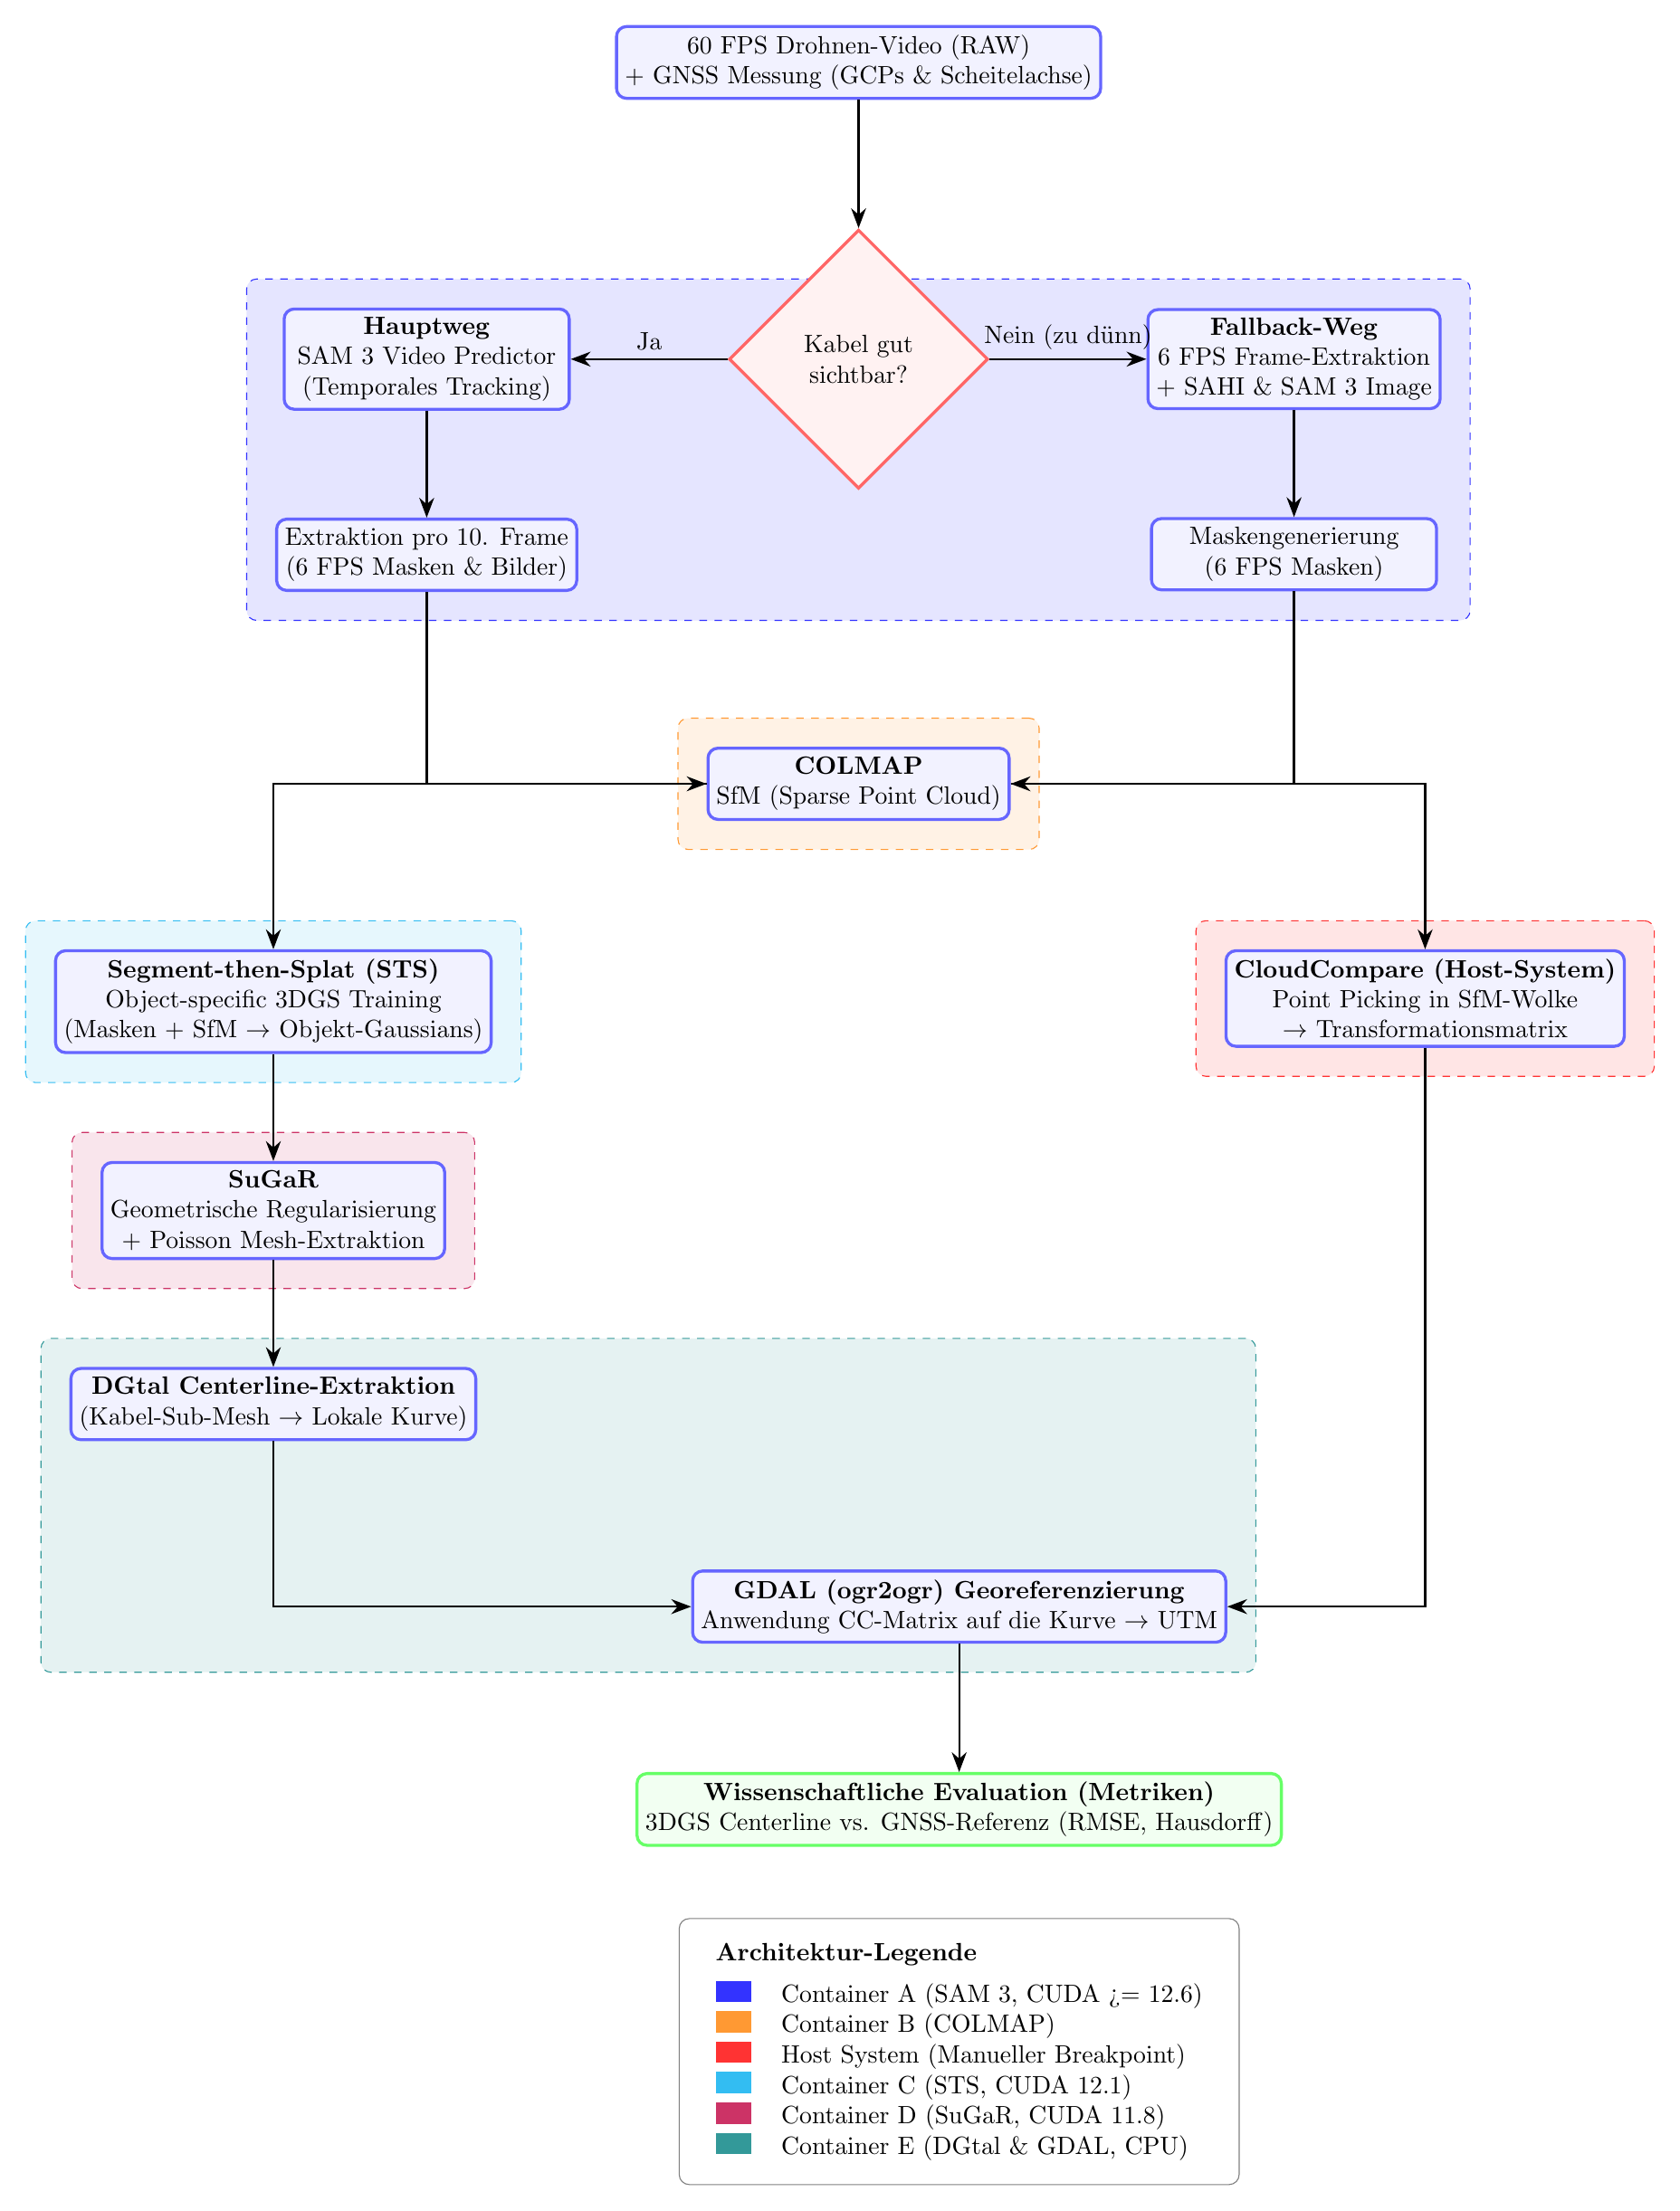
\begin{tikzpicture}[node distance=1.5cm, auto,
                box/.style={rectangle, draw=blue!60, fill=blue!5, very thick, minimum width=4cm, minimum height=1cm, align=center, rounded corners},
                decision/.style={diamond, draw=red!60, fill=red!5, very thick, text width=2.5cm, align=center},
                arrow/.style={-{Stealth[scale=1.2]}, thick},
                container_bg/.style={rectangle, draw, dashed, rounded corners, inner sep=0.4cm}]

            \node[box] (video) {60 FPS Drohnen-Video (RAW)\\+ GNSS Messung (GCPs \& Scheitelachse)};
            \node[decision, below=1.8cm of video] (check) {Kabel gut \\sichtbar?};
            \node[box, left=2.2cm of check] (pathA) {\textbf{Hauptweg}\\SAM 3 Video Predictor\\(Temporales Tracking)};
            \node[box, right=2.2cm of check] (pathB) {\textbf{Fallback-Weg}\\6 FPS Frame-Extraktion\\+ SAHI \& SAM 3 Image};

            \node[box, below=1.5cm of pathA] (extractA) {Extraktion pro 10. Frame\\(6 FPS Masken \& Bilder)};
            \node[box, below=1.5cm of pathB] (extractB) {Maskengenerierung\\(6 FPS Masken)};

            \node[box, below=3.6cm of check] (colmap) {\textbf{COLMAP}\\SfM (Sparse Point Cloud)};

            \node[box, below left=1.8cm and 3.0cm of colmap] (sts) {\textbf{Segment-then-Splat (STS)}\\Object-specific 3DGS Training\\(Masken + SfM $\rightarrow$ Objekt-Gaussians)};
            \node[box, below right=1.8cm and 3.0cm of colmap] (cc) {\textbf{CloudCompare (Host-System)}\\Point Picking in SfM-Wolke\\$\rightarrow$ Transformationsmatrix};

            \node[box, below=1.5cm of sts] (sugar) {\textbf{SuGaR}\\Geometrische Regularisierung\\+ Poisson Mesh-Extraktion};

            \node[box, below=1.5cm of sugar] (dgtal) {\textbf{DGtal Centerline-Extraktion}\\(Kabel-Sub-Mesh $\rightarrow$ Lokale Kurve)};

            \node[box, below right=1.8cm and 3.0cm of dgtal] (final) {\textbf{GDAL (ogr2ogr) Georeferenzierung}\\Anwendung CC-Matrix auf die Kurve $\rightarrow$ UTM};

            \node[box, draw=green!60, fill=green!5, below=1.8cm of final] (eval) {\textbf{Wissenschaftliche Evaluation (Metriken)}\\3DGS Centerline vs. GNSS-Referenz (RMSE, Hausdorff)};

            % Background containers
            \begin{pgfonlayer}{background}
                \node[container_bg, fill=blue!10, draw=blue!80, fit=(pathA) (pathB) (extractA) (extractB)] (contA) {};
                \node[container_bg, fill=orange!10, draw=orange!80, fit=(colmap)] (contB) {};
                \node[container_bg, fill=red!10, draw=red!80, fit=(cc)] (host) {};
                \node[container_bg, fill=cyan!10, draw=cyan!80, fit=(sts)] (contC) {};
                \node[container_bg, fill=purple!10, draw=purple!80, fit=(sugar)] (contD) {};
                \node[container_bg, fill=teal!10, draw=teal!80, fit=(dgtal) (final)] (contE) {};
            \end{pgfonlayer}

            % Legend
            \node[draw=black!50, fill=white, rectangle, rounded corners, anchor=north, inner sep=0.3cm, yshift=-1cm] at (eval.south) {
                \begin{tabular}{ll}
                    \multicolumn{2}{l}{\textbf{Architektur-Legende}}                                \\[1ex]
                    \textcolor{blue!80}{\rule{0.5cm}{0.3cm}}   & Container A (SAM 3, CUDA >= 12.6)  \\
                    \textcolor{orange!80}{\rule{0.5cm}{0.3cm}} & Container B (COLMAP)               \\
                    \textcolor{red!80}{\rule{0.5cm}{0.3cm}}    & Host System (Manueller Breakpoint) \\
                    \textcolor{cyan!80}{\rule{0.5cm}{0.3cm}}   & Container C (STS, CUDA 12.1)       \\
                    \textcolor{purple!80}{\rule{0.5cm}{0.3cm}} & Container D (SuGaR, CUDA 11.8)     \\
                    \textcolor{teal!80}{\rule{0.5cm}{0.3cm}}   & Container E (DGtal \& GDAL, CPU)   \\
                \end{tabular}
            };

            \draw[arrow] (video) -- (check);
            \draw[arrow] (check) -- node[above] {Ja} (pathA);
            \draw[arrow] (check) -- node[above] {Nein (zu dünn)} (pathB);
            \draw[arrow] (pathA) -- (extractA);
            \draw[arrow] (pathB) -- (extractB);
            \draw[arrow] (extractA) |- (colmap);
            \draw[arrow] (extractB) |- (colmap);
            \draw[arrow] (colmap) -| (sts);
            \draw[arrow] (colmap) -| (cc);
            \draw[arrow] (sts) -- (sugar);
            \draw[arrow] (sugar) -- (dgtal);
            \draw[arrow] (dgtal) |- (final);
            \draw[arrow] (cc) |- (final);
            \draw[arrow] (final) -- (eval);

        \end{tikzpicture}
    }
    \caption{Microservice-Architektur (v4): 5-Container-Pipeline mit Segment-then-Splat für objektspezifisches Training und SuGaR für geometrisches Meshing.}
\end{figure}

\section{Anhang: Single Source of Truth (SSOT) -- Pipeline Installation}
Dieses Dokument dient als zentrale Wahrheit (SSOT) für die Installation und Orchestrierung der gesamten 5-Container-Pipeline. Es fasst alle Hard- und Software-Abhängigkeiten zusammen, um Reproduzierbarkeit zu gewährleisten.

\subsection*{Hardware-Grundvoraussetzungen}
\begin{itemize}[noitemsep]
    \item \textbf{GPU:} CUDA-kompatible Nvidia GPU (Compute Capability 7.0+).
    \item \textbf{VRAM:} 24 GB (erforderlich, um in Paper-Evaluations-Qualität zu trainieren).
    \item \textbf{OS:} Windows 10/11 mit WSL2 oder natives Ubuntu Linux 22.04.
\end{itemize}

\subsection*{Container A: SAM 3 (Segmentierung)}
Zuständig für die 2D-Maskierung des Drohnenvideos. Dieser Container nutzt modernste Meta-Abhängigkeiten.

\textbf{Requirements (laut offizieller Vorgabe):}
\begin{itemize}[noitemsep]
    \item Python 3.10 or higher
    \item PyTorch 2.4 or higher (im Setup wird PyTorch mit der passenden CUDA-Laufzeitumgebung installiert)
    \item CUDA-kompatible GPU mit CUDA >= 12.6
\end{itemize}

\textbf{Implementierungsentscheidung: Docker vs. Conda}\\
Für die Ausführung der SAM 3.1 Codebasis wurde konzeptionell von einer reinen lokalen Conda-Umgebung Abstand genommen. Stattdessen läuft SAM 3.1 vollständig in einem dedizierten Docker-Container (\texttt{sam3-preprocess}).

\textbf{Gründe gegen Conda und für Docker:}
\begin{enumerate}[noitemsep]
    \item \textbf{CUDA-Konflikte:} SAM 3.1 verlangt moderne PyTorch-Versionen (z.\,B. 2.7.0 mit CUDA 12.6) und greift auf experimentelle C++ Extensions (\texttt{sam3\_cu}) zurück. In einer lokalen Anaconda-Umgebung kommt es hier mit den bestehenden CUDA 11.8 Treibern von COLMAP/SuGaR ständig zu "Layer Mismatches" und Kompilierungsfehlern. Docker kapselt die CUDA 12.6 Abhängigkeiten sauber vom Host-System ab.
    \item \textbf{Abhängigkeits-Knoten (Dependency Hell):} Das SAM 3.1 Release benötigt tiefgreifende Bibliotheken (\texttt{pycocotools}, \texttt{einops}, \texttt{timm}), die nativ im Container über \texttt{apt-get} und \texttt{pip} verlässlich zusammengestellt werden.
    \item \textbf{Hardware-Starvation (Host-Safety):} Das Laden von SAM 3.1 in Full-HD (\texttt{sam3.1\_multiplex.pt}) absorbiert immense RAM- und CPU-Ressourcen beim Instanziieren des Video-Predictors. Im Container können via \texttt{docker-compose.yml} die CPU-Berechnungen strikt gedrosselt werden (\texttt{OMP\_NUM\_THREADS=8}), um Systemabstürze effektiv zu verhindern. Ein VRAM- und RAM-Offloading ist zusätzlich im inferierenden Python-Skript konfiguriert.
    \item \textbf{Hugging Face Token-Sicherheit:} Über Docker-Secrets (\texttt{.env} / \texttt{HF\_TOKEN}) wird die Authentifizierung für Gated Models sicher gehandhabt, ohne lokale Systemumgebungen zu belasten.
\end{enumerate}

\textbf{Installationsablauf (Docker):}\\
Die Bereitstellung erfolgt vollautomatisch über das dedizierte \texttt{Dockerfile} auf Basis von \texttt{pytorch/pytorch:2.7.0-cuda12.6-cudnn9-devel}. Dies klont das offizielle Repository, baut die C++ Extensions und cacht über das Hugging Face Hub das 3.5\,GB schwere Multiplex-Gewicht persistent ins Host-Volume.

\textbf{Ausführung \& Masken-Export (Python API):}\\
Hier ist das Python-Skript zur temporalen Propagation des Kabel-Prompts im Video. Da der SAM 3 Video Predictor im Tracking-Modus aus Konsistenzgründen nur eine einzelne, eindeutige Maske pro Frame propagiert (und nicht die drei hierarchischen Skalen des Image Predictors), generiert das Skript die für das Curriculum-Learning von Segment-then-Splat (STS) benötigten Stufen (\texttt{small}, \texttt{middle}, \texttt{default}) künstlich über morphologische Bildoperationen (Erosion und Dilation):
\begin{verbatim}
import os
import cv2
import numpy as np
from PIL import Image
from sam3.model_builder import build_sam3_video_predictor

# 1. Video Predictor auf GPU 0 initialisieren
predictor = build_sam3_video_predictor(gpus_to_use=[0])

# 2. Session mit dem Drohnen-Video starten
video_path = "/data/video.mp4"
response = predictor.handle_request(
    request=dict(type="start_session", resource_path=video_path)
)
session_id = response["session_id"]

# 3. Prompt setzen (z. B. Punkt-Prompt auf das Kabel in Frame 0)
predictor.handle_request(
    request=dict(
        type="add_prompt",
        session_id=session_id,
        frame_index=0,
        points=[[1024, 768]],  # Beispielkoordinaten auf dem Kabel
        labels=[1]
    )
)

# 4. Stream-Propagation & Multi-Scale Export via Morphologie
output_dir = "/data/masks"
os.makedirs(output_dir, exist_ok=True)

# Definiere Kernel für Erosion und Dilation (Größe auf Kabeldurchmesser anpassen)
kernel = np.ones((5, 5), np.uint8)

# propagate_in_video liefert einen Generator
for response in predictor.handle_stream_request(
    request=dict(type="propagate_in_video", session_id=session_id)
):
    frame_idx = response["frame_index"]
    outputs = response["outputs"]
    obj_ids = outputs["out_obj_ids"]
    binary_masks = outputs["out_binary_masks"]  # Shape: [num_objects, H, W]

    # Erzeuge einen Unterordner pro Frame-Index
    frame_dir = os.path.join(output_dir, f"frame_{frame_idx:05d}")
    os.makedirs(frame_dir, exist_ok=True)

    for idx, obj_id in enumerate(obj_ids):
        mask = binary_masks[idx]  # Boolesches Array [H, W]
        if mask.any():
            # Konvertierung: True -> 255, False -> 0
            mask_uint8 = (mask * 255).astype(np.uint8)
            
            # 1. Middle (Original)
            img_middle = Image.fromarray(mask_uint8)
            img_middle.save(os.path.join(frame_dir, "middle.png"))
            
            # 2. Small (Erodiert für den stabilen Kabelkern)
            mask_small = cv2.erode(mask_uint8, kernel, iterations=1)
            img_small = Image.fromarray(mask_small)
            img_small.save(os.path.join(frame_dir, "small.png"))
            
            # 3. Default (Dilatiert für den Sicherheitsrand)
            mask_default = cv2.dilate(mask_uint8, kernel, iterations=1)
            img_default = Image.fromarray(mask_default)
            img_default.save(os.path.join(frame_dir, "default.png"))

# 5. Session sauber schließen
predictor.handle_request(
    request=dict(type="close_session", session_id=session_id)
)
\end{verbatim}

\subsection*{Container B: COLMAP (Structure from Motion)}
Generiert die Kameraposen und die Sparse Point Cloud aus den maskierten Drohnenbildern.
Aufgrund der massiven Architekturänderungen (Einführung von GLOMAP) in Release 4.0.0, wird explizit zur stabileren Patch-Version \textbf{4.0.4} geraten, welche kritische Bugs (Speicherlecks, Race-Conditions in der Datenbank) behebt.

\textbf{Quellen \& Docker-Image:}
\begin{itemize}[noitemsep]
    \item \textbf{Releases:} \url{https://github.com/colmap/colmap/releases}
    \item \textbf{Docker-Image:} \texttt{docker pull colmap/colmap:4.0.4-cuda}
\end{itemize}

\textbf{Ausführung \& PLY-Export (für CloudCompare):}\\
Da COLMAP die Punktwolke standardmäßig in einem proprietären Binärformat (\texttt{.bin}) speichert, welches von CloudCompare nicht direkt gelesen werden kann, wird die Punktwolke direkt im Anschluss an die Rekonstruktion über den \texttt{model\_converter} in eine standardisierte \texttt{.ply}-Datei exportiert. Um eine geometrische Verformung der Punktwolke (ebene Entartung/Kollaps) während der Rekonstruktion unkalibrierter Drohnenbilder zu verhindern, wird die Parametrisierung basierend auf modernsten Photogrammetrie-Workflows angepasst (\texttt{SIMPLE\_RADIAL} Kameramodell, erzwungenes gemeinsames Objektiv via \texttt{single\_camera 1} und sequentielles Matching).

\begin{verbatim}
# 1. Feature-Extraktion (Kameramodell einschränken & gleiches Objektiv forcieren)
colmap feature_extractor \
    --database_path /data/scene/database.db \
    --image_path /data/scene/images \
    --ImageReader.camera_model SIMPLE_RADIAL \
    --ImageReader.single_camera 1

# 2. Keypoint-Matching (Sequentiell mit Overlap statt Exhaustive für Videoüberhang)
colmap sequential_matcher \
    --database_path /data/scene/database.db \
    --SequentialMatching.overlap 15

# 3. Structure-from-Motion (Sparse Reconstruction)
mkdir -p /data/scene/sparse
colmap mapper \
    --database_path /data/scene/database.db \
    --image_path /data/scene/images \
    --output_path /data/scene/sparse

# 4. Export der Punktwolke als PLY-Format
colmap model_converter \
    --input_path /data/scene/sparse/0 \
    --output_path /data/scene/sparse/points3D.ply \
    --output_type PLY
\end{verbatim}

\textbf{Hintergrund zur mathematischen Optimierung (für „Dummis“ erklärt):}\\
Wenn wir ein Drohnenvideo Frame-für-Frame in COLMAP einspeisen, stehen wir vor zwei massiven mathematischen Hürden:
\begin{enumerate}[noitemsep]
    \item \textbf{Die Overfitting-Falle (Zu viele Freiheitsgrade):} Wenn wir COLMAP ein extrem komplexes Kameramodell (wie \texttt{OPENCV}) geben, versucht der Algorithmus, für jedes der hunderte Bilder Brennweiten und Objektivkrümmungen völlig unabhängig voneinander zu schätzen. Das führt zu einer geometrischen Katastrophe: COLMAP „schummelt“ mathematisch, verbiegt die Parameter extrem und presst die gesamte 3D-Welt flach wie eine Flunder auf eine einzige Ebene zusammen, um Restfehler zu minimieren. Mit \texttt{SIMPLE\_RADIAL} verbieten wir diese Schummelei, indem wir nur noch vier physikalische Kern-Parameter zulassen. Gleichzeitig zentrieren wir über \texttt{--ImageReader.single_camera 1} alle Rechnungen auf genau \textit{ein} einziges, geteiltes Objektiv.
    \item \textbf{Die Basislinien-Falle (Fast-parallele Sehstrahlen):} Wenn zwei aufeinanderfolgende Bilder nur Millisekunden auseinander liegen, bewegt sich die Drohne kaum fort. Die Sehstrahlen der Kameras schneiden sich unter einem extrem spitzen Winkel ($0^\circ$). COLMAP kann die Tiefe dadurch nicht verlässlich berechnen und flacht die Punktwolke ab. Indem wir über \texttt{SAM3_FRAME_STEP} künstlich nur jedes z.\,B. 5. oder 10. Bild rekonstruieren, vergrößern wir den physischen Abstand (die Basislinie) zwischen den Kamera-Standorten. Dadurch schneiden sich die Sehstrahlen in einem gesunden, steilen Dreieck und zaubern eine plastische, tiefe, dreidimensionale 3D-Struktur hervor.
    \item \textbf{Die Treffsicherheits-Falle (Falsche Übereinstimmungen):} Das standardmäßige \texttt{exhaustive\_matcher} vergleicht jedes Bild mit absolut jedem anderen Bild. Bei sich wiederholenden Texturen (z.\,B. Gleisen, Rohren oder Asphaltmustern) führt das zu fatalen Fehlverknüpfungen (False Loop Closures). Indem wir auf den \texttt{sequential\_matcher} mit einem Overlap von 15 Frames umschalten, vergleicht COLMAP Bilder nur noch mit ihren unmittelbaren zeitlichen Nachbarn (im Video naheliegend). Das ist nicht nur hunderte Male schneller, sondern schützt die 3D-Punktwolke hochgradig effektiv vor geometrischer Verwerfung.
    \item \textbf{Die CLI-Versions-Falle (Veraltete Befehle):} Beim Upgrade auf modernere, offizielle Docker-Images (wie \texttt{colmap/colmap:latest} ab Version \texttt{4.0}) scheitern klassische, ältere Skripte an deprecated Parametern. Parameter wie \texttt{--SiftExtraction.use_gpu} oder \texttt{--SiftExtraction.max_image_size} wurden aus dem CLI-Befehlssatz gestrichen, da die moderne CUDA-Hardware-Beschleunigung und das Auto-Resizing heute vollautomatisch und optimal aufeinander abgestimmt nativ im Kernel von COLMAP implementiert sind. Das Entfernen dieser Parameter garantiert die reibungslose Ausführung auf modernen GPGPU-Knoten.
\end{enumerate}

\textit{Breakpoint:} Nach diesem Schritt pausiert das Master-Skript automatisch. Die erzeugte Datei \texttt{points3D.ply} wird auf dem Host-System in CloudCompare geladen, um die manuelle Georeferenzierung via GCP-Point-Picking durchzuführen. Nach dem Speichern der Transformationsmatrix wird das Skript fortgesetzt.

\subsection*{Container C: Segment-then-Splat (Object-specific 3DGS)}
Führt das objektspezifische 3DGS-Training durch. STS weist jedem initialen COLMAP-Gaussian eine Object-ID zu (basierend auf den SAM 3 Masken) und trainiert mit dem nativen Object-specific Loss ($\mathcal{L}_{obj}$). Das intern vorgesehene AutoSeg-SAM2 wird vollständig deaktiviert und durch die externen SAM 3 Masken aus Container A ersetzt. Hierfür wird der Dataloader (z. B. in \texttt{scene/dataset\_readers.py} oder \texttt{scene/cameras.py}) so angepasst, dass er pro Frame die drei Masken-Dateien (\texttt{small.png}, \texttt{middle.png}, \texttt{default.png}) einliest und in das Dictionary \texttt{viewpoint\_cam.object\_masks} einspeist.

\textbf{Requirements (Docker-Umgebung):}
\begin{itemize}[noitemsep]
    \item \textbf{Base Image:} \texttt{nvidia/cuda:12.1.0-devel-ubuntu22.04}
    \item Python 3.10, PyTorch 2.3.1 mit CUDA 12.1
    \item 24 GB VRAM
\end{itemize}

\textbf{Installationsablauf:}
\begin{verbatim}
git clone https://github.com/luyr/Segment-then-Splat --recursive
cd Segment-then-Splat

conda create -n segment_then_splat python=3.10
conda activate segment_then_splat
pip install torch==2.3.1 torchvision==0.18.1 torchaudio==2.3.1 \
    --index-url https://download.pytorch.org/whl/cu121
pip install -r requirements.txt --no-build-isolation
\end{verbatim}

\textbf{Anpassung des Dataloaders und Trainingsablauf:}
Im Datensatz-Reader wird die folgende Logik implementiert, um die Maskentensoren direkt zu laden:
\begin{verbatim}
# Pseudo-Code zur Anpassung des Kamera-Ladevorgangs:
import torch
from PIL import Image

def load_object_masks(frame_dir):
    scales = ["small", "middle", "default"]
    object_masks = {}
    for scale in scales:
        mask_path = os.path.join(frame_dir, f"{scale}.png")
        if os.path.exists(mask_path):
            # Graustufen laden, Normalisieren und als Boolean-Tensor konvertieren
            mask_img = Image.open(mask_path).convert("L")
            mask_np = np.array(mask_img) > 127
            mask_tensor = torch.from_numpy(mask_np).bool() # Shape: [H, W]
            object_masks[scale] = [mask_tensor]
        else:
            object_masks[scale] = []
    return object_masks

# Zuweisung zur viewpoint_cam während der Szenen-Initialisierung:
# viewpoint_cam.object_masks = load_object_masks(f"/data/masks/frame_{frame_idx:05d}")
\end{verbatim}

\textbf{Ausführung des Trainings:}
\begin{verbatim}
# 1. Object-specific Initialization (Zuweisung der initialen SfM-Punkte)
# STS prüft anhand der default/middle/small Masken die Punkt-Sichtbarkeiten
python ./helpers/object_specific_initialization.py \
    --scene_root /data/scene/

# 2. Training mit dem geänderten Dataloader und Object-specific Loss
python train.py -s /data/scene/ -m /data/output \
    --eval --iterations 40000 \
    --num_sample_objects 3 \
    --densify_until_iter 20000 \
    --partial_mask_iou 0.3
\end{verbatim}

\textbf{Wichtiger Hinweis:} Durch die Entkopplung der Maskenberechnung läuft die CUDA-spezifische Optimization in Container C völlig autark von den CUDA-Anforderungen des SAM 3 Frontends in Container A.

\subsection*{Container D: SuGaR (Geometrische Regularisierung \& Meshing)}
Lädt den vortrainierten STS-Checkpoint und wendet die geometrische Regularisierung (DN-Consistency, Normal Alignment) sowie Poisson Surface Reconstruction an. Dies ist der sensitivste Container bezüglich CUDA-Versionen.

\textbf{Exkurs: Conda innerhalb von Docker}\\
Obwohl Docker bereits das Betriebssystem isoliert und Conda somit theoretisch redundant wäre, wird Miniconda in diesem Container explizit genutzt. Der Grund: 3DGS-Repositories (wie SuGaR) setzen stark auf vorkompilierte Conda-Binaries (z.B. \texttt{pytorch-cuda}) und exakte Paket-Versionen. Durch die strikte Nutzung von Conda im Docker-Container werden fatale C++ Kompilierungsfehler beim Rasterizer-Modul präventiv vermieden.

\textbf{Requirements (Docker-Umgebung):}
\begin{itemize}[noitemsep]
    \item \textbf{Base Image:} \texttt{nvidia/cuda:11.8.0-devel-ubuntu22.04} (Dieses Image bringt das kompatible CUDA 11.8 SDK direkt mit).
    \item \textbf{C++ Compiler:} Installation via \texttt{apt-get install build-essential} (installiert GCC/G++, was unter Linux Visual Studio ersetzt und garantiert mit CUDA 11.8 kompatibel ist).
    \item 24 GB VRAM (erforderlich, um in Paper-Evaluations-Qualität zu trainieren).
\end{itemize}

\textbf{Installationsablauf (Dockerfile-Struktur):}
\begin{verbatim}
# 1. Base Image mit CUDA 11.8 & GCC
FROM nvidia/cuda:11.8.0-devel-ubuntu22.04

# 2. System-Abhängigkeiten installieren
ENV DEBIAN_FRONTEND=noninteractive
RUN apt-get update && apt-get install -y \
    build-essential \
    git \
    wget \
    curl \
    libgl1-mesa-glx \
    libglib2.0-0 \
    && rm -rf /var/lib/apt/lists/*

# 3. Miniconda installieren
RUN wget https://repo.anaconda.com/miniconda/Miniconda3-latest-Linux-x86_64.sh -O miniconda.sh && \
    bash miniconda.sh -b -p /opt/conda && \
    rm miniconda.sh
ENV PATH=/opt/conda/bin:$PATH

# 4. Conda Environment anlegen und Shell konfigurieren
RUN conda create --name sugar -y python=3.9
SHELL ["conda", "run", "-n", "sugar", "/bin/bash", "-c"]

# 5. PyTorch & CUDA 11.8 Bibliotheken installieren
RUN conda install pytorch==2.0.1 torchvision==0.15.2 torchaudio==2.0.2 \
    pytorch-cuda=11.8 -c pytorch -c nvidia -y && \
    conda install -c fvcore -c iopath -c conda-forge fvcore iopath -y && \
    conda install pytorch3d==0.7.4 -c pytorch3d -y && \
    conda install -c plotly plotly -y && \
    conda install -c conda-forge rich plyfile==0.8.1 jupyterlab nodejs ipywidgets -y

# 6. Repositories klonen und Submodule kompilieren
WORKDIR /workspace
RUN git clone https://github.com/Anttwo/SuGaR.git && \
    cd SuGaR && \
    pip install open3d PyMCubes && \
    pip install -e . && \
    cd gaussian_splatting/submodules/diff-gaussian-rasterization/ && \
    pip install -e . && \
    cd ../simple-knn/ && \
    pip install -e .

# Conda-Umgebung im PATH systemweit als Standard setzen
ENV PATH=/opt/conda/envs/sugar/bin:$PATH
\end{verbatim}

\textbf{Details zur Build-Dauer und Kompilierungskomplexität (Container D):}\\
In der praktischen Umsetzung stellte der Docker-Build für SuGaR eine signifikante Hürde dar, die mehrere Optimierungszyklen erforderte:
\begin{enumerate}[noitemsep]
    \item \textbf{Explizite CUDA-Architektur-Spezifikation (\texttt{TORCH\_CUDA\_ARCH\_LIST}):} Um die Ausführbarkeit auf einer breiten Hardwarelandschaft (z.\,B. RTX 30er, 40er, Server-GPUs) abzusichern, mussten mehrere CUDA-Architekturen (\texttt{"7.0;7.5;8.0;8.6;8.9;9.0"}) explizit beim Build hinterlegt werden. Der NVCC-Compiler kompiliert die C++ Extensions von \texttt{diff-gaussian-rasterization} und \texttt{simple-knn} für jede Architektur einzeln, was die Kompilierungszeit erheblich verlängert.
    \item \textbf{Conda-Umgebung und Build-Isolation (\texttt{-{}-no-build-isolation}):} Standardmäßig isoliert \texttt{pip} Builds in temporären virtuellen Umgebungen. Weil darin jedoch kein Zugriff auf die installierten PyTorch- und CUDA-Laufzeitbibliotheken von Conda besteht, kommt es zu fatalen Kompilierungsabbrüchen (z.\,B. bzgl. fehlender \texttt{torch}-Vektoren). Erst durch Hinzufügen von \texttt{-{}-no-build-isolation} greift der Build-Prozess direkt auf den vorkonfigurierten Conda-Compiler-Stack zu.
    \item \textbf{Parallelisierung via \texttt{ninja-build}:} Ohne eine parallele Kompilierungssteuerung fallen manche Python-Installer auf serielle Single-Thread-Kompilierung zurück, was zu extremen Timeouts oder Speicherüberläufen führt. Das Vorinstallieren des systemweiten Compilers \texttt{ninja-build} im Docker-Base-Image ermöglichte hierbei die maximal parallele Lastverteilung auf alle CPU-Kerne.
\end{enumerate}

\textbf{Automatisierte Punktwolkenfilterung zur Rauschminimierung (\texttt{filter\_cable\_pc.py}):}\\
Ein schwerwiegender konzeptioneller Fehler bei der direkten Rekonstruktion mittels SuGaR ist die unkontrollierte Generierung von Hintergrund-Splats. SuGaR besitzt keine eingebaute Logik, Hintergrundbereiche zu verwerfen -- ohne Filter arbeitet der Algorithmus an einer dichten Punktwolke des gesamten Raumes. Ein eigens implementiertes Python-Hilfsprogramm \texttt{filter\_cable\_pc.py} wurde als Bindeglied (Scheduler Schritt 3.5) zwischen Phase 3 und Phase 4 geschaltet:
\begin{itemize}[noitemsep]
    \item \textbf{Funktionsweise:} Das Skript parst den binären PLY-Header des STS-Outputs und liest die Segmentierungs-Vektoren aus. Zu jedem 3D-Gaussian existieren die durch STS zugewiesenen Objektspalten (\texttt{obj\_id\_s}, \texttt{obj\_id\_m}, \texttt{obj\_id\_l}). 
    \item \textbf{Selektive Extraktion:} Über das Argument \texttt{-{}-level m} und \texttt{-{}-object\_id 1} wählt das Skript gezielt nur die Datenzeilen aus, die der mittleren Kategorie der Kabeltrasse entsprechen (Kabel = ID 1, Hintergrund = ID 0). Alle unkorrelierten Raumpunkte werden vollständig aus den Vektormatrizen gelöscht.
    \item \textbf{Fallback-Mechanismus:} Code-Fehler oder leere Segmente fängt das Skript über einen automatischen Fallback-Prüfschritt ab. Sollte das gefilterte Segment exakt 0 Punkte liefern (z.\,B. durch vertauschte Klassenindizes im Trainingslauf), greift die Logik selbstständig auf alle nicht-leeren Masken zurück oder reicht die Originalpunktwolke durch, um ein Abbrechen der Pipeline im Batch-Lauf zu verhindern.
\end{itemize}
Durch diesen Filter-Lauf wird verhindert, dass SuGaR Millionen ungenutzter schwarzer Gaussians (sog. \textit{Floating Artifacts}) in den leeren Raum außerhalb des Kabelgrabens hineinrechnet.

\textbf{Wichtige Best-Practices \& Parameter-Tuning (SuGaR):}\\
Für qualitativ hochwertige Rekonstruktionen (insb. dünne Kabelstrukturen) sind folgende Parameter entscheidend (siehe \href{https://github.com/Anttwo/SuGaR}{SuGaR Tips}):
\begin{itemize}[noitemsep]
    \item \textbf{Regularisierung:} Nutze zwingend \texttt{-r "dn\_consistency"} für die beste Mesh-Qualität.
    \item \textbf{Löcher im Mesh:} Wenn die Mesh-Bereinigung zu aggressiv ist, setze \texttt{vertices\_density\_quantile = 0.} in \texttt{sugar\_extractors/coarse\_mesh.py}.
    \item \textbf{Ellipsoide Artefakte (Bumps):} Reduziere die Poisson-Tiefe \texttt{poisson\_depth} (z.B. von 10 auf 7 oder 8 in \texttt{coarse\_mesh.py}), falls einzelne Gaussians sichtbar werden.
    \item \textbf{Große Szenen:} Bei weiten Distanzen sollten Custom Bounding Boxes (\texttt{--bboxmin} und \texttt{--bboxmax}) genutzt werden, um die Extraktion zu fokussieren.
\end{itemize}


\subsection*{Container E: DGtal \& GDAL (Post-Processing)}
Führt die Extraktion der Centerline auf dem isolierten Kabel-Sub-Mesh durch und überführt diese in georeferenzierte GIS-Formate (GeoJSON). Da \texttt{DGtal} eine komplexe C++ Bibliothek mit zahlreichen Abhängigkeiten (Eigen, CGAL, ITK) ist, wird direkt auf dem offiziellen \texttt{dgtal:latest} Docker-Image aufgebaut.

\textbf{Requirements \& Repositories:}
\begin{itemize}[noitemsep]
    \item \textbf{DGtal Release (v2.1):} \url{https://github.com/DGtal-team/DGtal/releases/tag/v2.1}
    \item \textbf{GDAL:} \url{https://github.com/OSGeo/gdal}
    \item \textbf{OGR2OGR Wrapper:} \url{https://github.com/wavded/ogr2ogr}
\end{itemize}

\textbf{Docker Build \& Ausführung:}
\begin{verbatim}
# Offizielles DGtal Image bauen (im DGtal Repo Ordner)
docker build -t dgtal:latest .

# Nachinstallation von GDAL (ogr2ogr) und Python-Paketen über ein abgeleitetes Dockerfile
FROM dgtal:latest
USER root
RUN apt-get update && apt-get install -y gdal-bin libgdal-dev python3-pip python3-numpy && \
rm -rf /var/lib/apt/lists/*
USER digital

# Interaktive Ausführung mit Bind-Mount
docker run -it -v /host/path/data:/data --user=digital dgtal-gdal:latest bash
cd /home/digital/git/DGtal/build/examples
# 1. DGtal Centerline-Extraktion auf dem lokalen Kabel-Mesh ausführen
# (Erzeugt /data/centerline_local.csv)

# 2. Ausführen des Python-Skripts zur Georeferenzierung
# (Wendet 4x4-Transformationsmatrix an und addiert UTM-Koordinaten des Anker-GCPs automatisch)
python /data/scripts/transform_centerline.py \
    --input_csv /data/centerline_local.csv \
    --matrix /data/matrix.txt \
    --anchor_txt /data/01_raw/anchor.txt \
    --output_csv /data/centerline_utm.csv

# 3. Konvertierung des UTM-Ergebnisses in standardisiertes GeoJSON (EPSG:25832)
ogr2ogr -f "GeoJSON" /data/centerline.geojson /data/centerline_utm.csv -a_srs EPSG:25832
\end{verbatim}

\end{document}
